\chapter{Results and Discussion} 
% Main chapter title
\label{Chapter2} 
\section{Synthesis of Novel Nanostructures}
\subsection{Modification of Synthetic Route}
The synthesis of the target compounds is outlined in Figure \ref{C16-Ala-Lys_synthesis}. It employs a series of Boc-protection, TBTU-mediated peptide coupling and Boc-deprotection steps. All target compounds were characterised by \textsuperscript{1}H, \textsuperscript{13}C and DEPT-135 NMR, as well as MS and IR, as outlined in the experimental (Chapter \ref{Chapter5}).

The original protocol for the synthesis of C\textsubscript{16}-Gly-D/L-Lys family of nanoscale heparin binders originally published by Chan, Laurini \textit{et al.}, was found to not work well for the synthesis of this new family of heparin binders after the glycine group was replaced by alanine.\textsuperscript{\cite{Chan2016ChiralBinding}} In the coupling step to join the amino acid to the C\textsubscript{16} carbon chain, as shown in Figure \ref{C16-Ala-Lys_synthesis}, the original method has the reactants being dissolved in dichloromethane (DCM), but on removing solvent \textit{in vacuo}, the residue is redissolved into ethyl acetate, before washing the organic layer.  The paper gives an observed yield of 40\% for both enantiomers. In comparison, using this method for the synthesis of C\textsubscript{16}-Ala(Boc) this observed yield falls to only 22\%. 

After discussion with coworkers, it was decided to change the solvent for this washing step from ethyl acetate to DCM. Modifying the solvent used here caused the yield to rise dramatically (L: 51 \%; D: 68 \%), giving a much more substantial amount of product after this step and thus permitting further synthesis at scale. 

On searching the literature, it was discovered that this behaviour is already known i.e. changing the amino acid changes the solubility of a compound in a given solvent. According to Needham \textit{et al.}, glycine as an amino acid is much more soluble than alanine in all of the solvent systems that were tested.\textsuperscript{\cite{Needham1971SolubilitySystems}}
Therefore, the effect that changing the solvent had on yield is not surprising, and shows that the original issue with the low yield was due to the C\textsubscript{16}-Ala(Boc) not being sufficiently soluble in the solvent and instead forming a suspension.  It is then likely that some of the product was lost when the layers were separated after the addition of NaHSO\textsubscript{4}. 

From previous work by Smith and coworkers, it is well known that small changes in these systems cause dramatic changes in their properties and behaviour. Chan reported that inserting a glycine spacer between the lysine binding group and carbon chain introduced chiral selectivity towards both heparin and DNA, whilst Vieira noted that changing the length of the hydrophobic carbon chain altered the solubility in aqueous media and also affects their ability to self-assemble, finally Albanyan stated that the inclusion of alkene groups within the hydrophobic carbon chain influences the size of the SAMul nanostructures.\textsuperscript{\cite{Chan2016ChiralBinding,Vieira2017EmergenceHeparin,Albanyan2017Self-AssembledLigands}} 

\newpage
\begin{figure}[ht!]
\centering{
\includegraphics[scale=0.96]{Figures/Synthesis_of_C16-L-Ala-L-Lys_V2.eps}}
\caption{Modified synthetic route used to synthesise the novel heparin binding nanostructures}
\label{C16-Ala-Lys_synthesis}
\end{figure}
\newpage

\subsection{TBTU-Mediated Peptide Coupling}
The synthetic route shown in Figure \ref{C16-Ala-Lys_synthesis} employs a sequence of Boc protection and deprotection steps. This is achieved by the use of Boc anhydride (di-tert-butyldicarbonate), to introduce the Boc protecting group onto the amine moiety. This technique is used to confer regioselectivity onto the TBTU-mediated peptide coupling steps, the mechanism of which is shown in Figure \ref{TBTU mechanism}, by blocking the reactive amine, and preventing self-polymerisation of the amino acid. This forces the reaction to take place by first removing a proton from the carboxylic acid group, and further reaction with TBTU activates the carboxylic acid derivative.\textsuperscript{\cite{Valeur2009AmideReagents}} The activated carboxylic acid derivative then reacts with the amine group of the other reagent, in this case C\textsubscript{16}-Ala. 

\subsection{Hygroscopic Properties of Lysine}
Whilst carrying out the synthesis of the products outlined above, it was noticed that some of the products appeared to be hygroscopic and others were not. 
The property that the hygroscopic products had in common is that they all contain a lysine group. Consequently, C\textsubscript{16}-D-Ala-D-Lys and L-Lys(Boc)\textsubscript{2} are hygroscopic, whilst C\textsubscript{16}-D-Ala(Boc) is not. 
The lysine group introduces this property because lysine is a significantly more polar amino acid. 

It is known that charged compounds make stable hydrates when exposed to water, hence the affinity of the lysine group for water within the atmosphere and the hygroscopic behaviour that has been seen. Reaction conditions have not been changed because of this behaviour, but it does cause issues with handling these products, as they absorb water rapidly on being exposed to air. Consequently, they are stored under a nitrogen atmosphere, with lids wrapped tightly in parafilm before being frozen. 
\newpage

\begin{figure}[ht!]
\centering
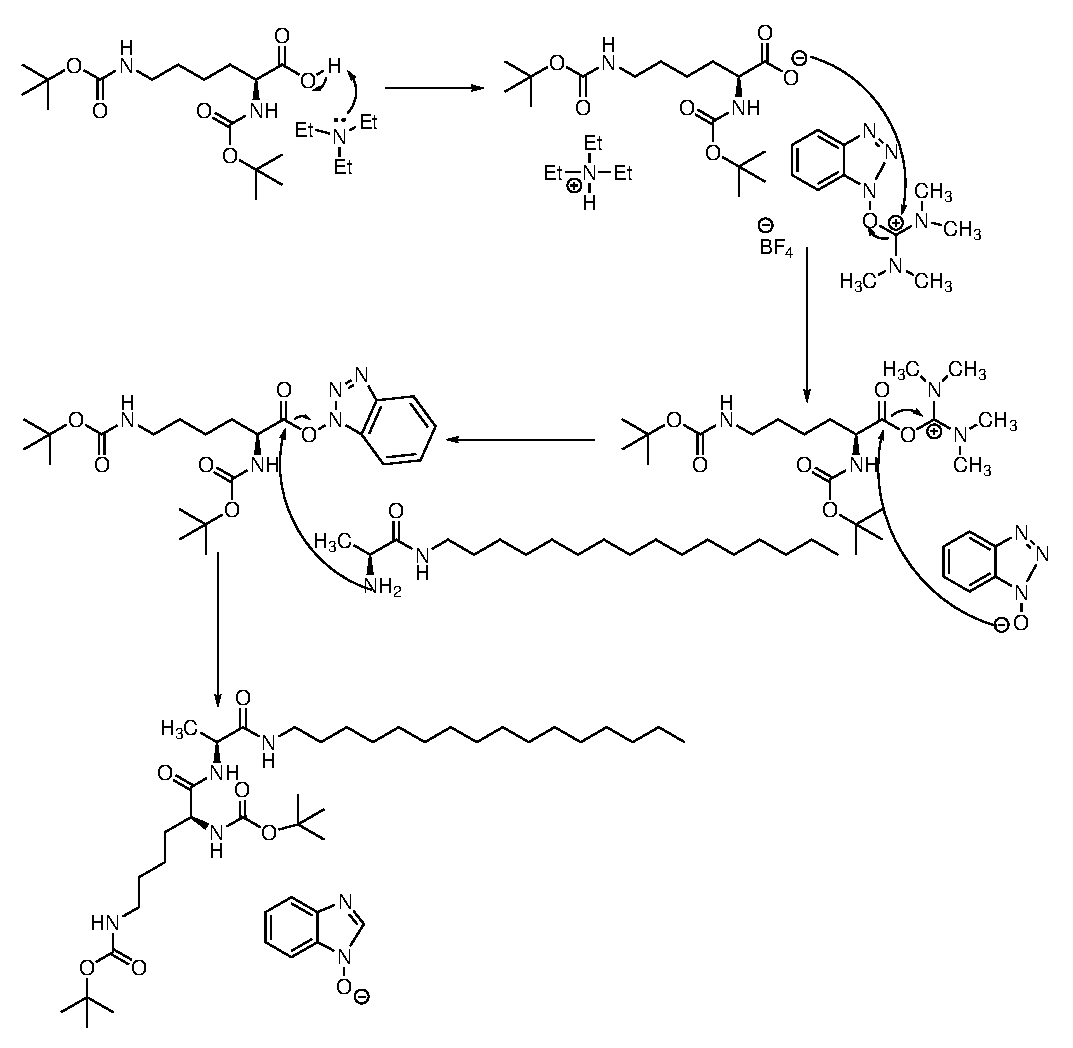
\includegraphics[scale=0.9]{Figures/TBTU_mechanism.eps}
\caption{Mechanism for TBTU mediated peptide coupling}
\label{TBTU mechanism}
\end{figure}
\newpage
\subsection{Adding and Removing Boc-Protecting Groups}
Boc protecting groups are used in this synthesis to generate regioselectivity in the reaction, which then results in only one isomer of product being formed. This has been achieved using Boc anhydride and sodium hydroxide as the base. The mechanism for this is shown in Figure \ref{Boc_protection}. 
\begin{figure}[ht!]
\centering
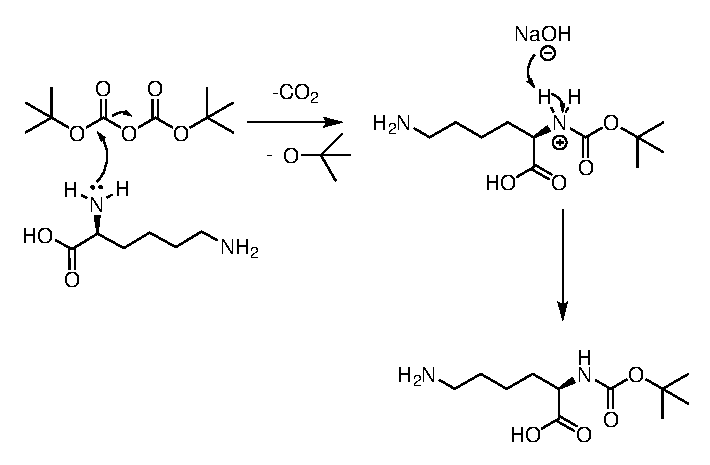
\includegraphics[scale=1]{Figures/Boc_protection.eps}
\caption{Mechanism for Boc protection of L-Ala. Only Boc- protection for one of the NH\textsubscript{2} groups is shown.}
\label{Boc_protection}
\end{figure}

Once the reaction is complete and the desired product has been formed, the protecting groups are no longer useful and need to be removed. There are a variety of ways in which this can be done, but for Boc-deprotection, this reaction is always acid mediated  (Figure \ref{Boc_deprotection}).
\begin{figure}[ht!]
\centering
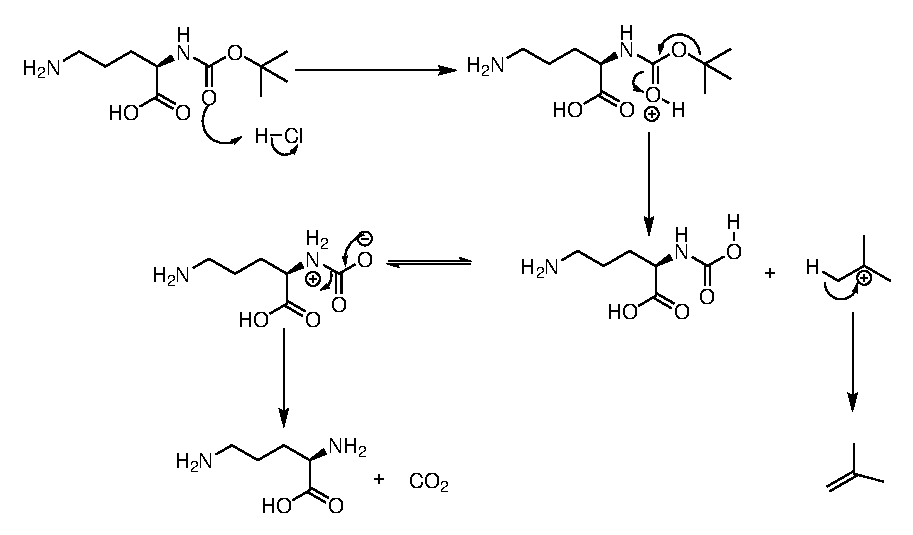
\includegraphics[scale=1]{Figures/Boc_deprotection.eps}
\caption{Mechanism for Boc-deprotection of L-Ala(Boc). Only Boc-deprotection for one NH\textsubscript{2} group is shown.From \cite{Clayden2012OrganicChemistry}} 
\label{Boc_deprotection}
\end{figure}
\newpage
In this work, both dissolving the Boc-protected product in solvent (usually DCM or MeOH), then bubbling HCl gas through the solvent, and dissolving the Boc-protected product into 15 eq. 4 M HCl in dioxane have been used.\footnote{This change is not due to the compounds, but purely due to a limited supply of HCl gas. The author however does have a preference for using 4M HCl in dioxane as this appears to be easier to use.}

Figures \ref{KAT1.16_NMR} and \ref{KAT1.17_NMR} show the effect of dissolving the Boc-protected product 4 M HCl in dioxane, then stirring the solution for one hour. 
Both of these techniques are successful at removing the Boc protecting group - with loss of the \textsuperscript{1}H NMR peak at 1.45 ppm, which corresponds to the Boc group.

\begin{figure}[ht!]
\centering
\includegraphics[scale=0.47]{NMR/KAT1_16.pdf}
\caption{\textsuperscript{1}H NMR C\textsubscript{16}-L-Ala(Boc)}
\label{KAT1.16_NMR}
\end{figure}
\begin{figure}[ht!]
\centering
\includegraphics[scale=0.47]{NMR/KAT1_17.pdf}
\caption{\textsuperscript{1}H NMR of C\textsubscript{16}-L-Ala after removal of Boc-protecting group using 4 M HCl in dioxane}
\label{KAT1.17_NMR}
\end{figure}

\newpage
\subsection{NMR Analysis of Target Compounds}
The four target compounds - C\textsubscript{16}-L-Ala-L-Lys, C\textsubscript{16}-L-Ala-D-Lys, C\textsubscript{16}-D-Ala-L-Lys and C\textsubscript{16}-D-Ala-D-Lys have all been successfully synthesised. These constitute two enantiomeric pairs of binders which have a diastereomeric relationship to each other. The \textsuperscript{1}H NMR spectra are presented in Figures \ref{KAT1.19_NMR} to \ref{KAT1.30_NMR}. 

These NMR spectra are broadly similar to each other; as would be expected. Key proton resonances all appear at equivalent ppm values (Table \ref{NMR_shift}). However, it is clear that the coupling patterns of the CH\textsubscript{2}-N protons are somewhat more complex for the homochiral pair (L,L/D,D) in comparison to the heterochiral pair (L,D/D,L). which is most apparent for the resonances at ca. 3.1 ppm. This reflects the diastereomeric relationship of these two pairs of compounds, leading to differences in coupling, possibly induced by conformational differences between the molecules, leading to subsequent change in torsion angle between coupled protons. 
\newline
\begin{table}[h!]
\centering
\caption{A summary of the differences of chemical shift in \textsuperscript{1}H NMR, between the four target compounds}
\begin{tabular}{l|l|l|l|l}
\textbf{Compound Name} & \textbf{Ala (CH) \textdelta}  & \textbf{Lys (CH) \textdelta} & \textbf{CH\textsubscript{2}-j \textdelta} & \textbf{CH\textsubscript{2}-b \textdelta} \\
\hline
\textbf{C\textsubscript{16}-L-Ala-L-Lys} & 4.31 & 3.91  & 3.12 & 2.97 \\
\textbf{C\textsubscript{16}-D-Ala-D-Lys} & 4.29 & 3.90 & 3.15 & 2.95 \\
\textbf{C\textsubscript{16}-D-Ala-L-Lys} & 4.32 & 3.92 & 3.17 & 2.95 \\
\textbf{C\textsubscript{16}-L-Ala-D-Lys} & 4.32 & 3.92 & 3.17 & 2.97\\
\end{tabular}
\label{NMR_shift}
\end{table}

\newpage
\begin{figure}[ht!]
\centering
\includegraphics[scale=0.47]{NMR/KAT1_19.pdf}
\caption{\textsuperscript{1}H NMR of C\textsubscript{16}-L-Ala-L-Lys}
\label{KAT1.19_NMR}
\end{figure}

\begin{figure}[ht!]
\centering
\includegraphics[scale=0.47]{NMR/KAT1_35.pdf}
\caption{\textsuperscript{1}H NMR of C\textsubscript{16}-D-Ala-D-Lys}
\label{KAT1.35_NMR}
\end{figure}

\begin{figure}[ht!]
\centering
\includegraphics[scale=0.47]{NMR/KAT1_22.pdf}
\caption{\textsuperscript{1}H NMR of C\textsubscript{16}-D-Ala-L-Lys}
\label{KAT1.22_NMR}
\end{figure}

\newpage
\begin{figure}[ht!]
\centering
\includegraphics[scale=0.47]{NMR/KAT1_30.pdf}
\caption{\textsuperscript{1}H NMR of C\textsubscript{16}-L-Ala-D-Lys}
\label{KAT1.30_NMR}
\end{figure}

\begin{table}[h!]
\centering
\caption{A summary of the differences of chemical shift in \textsuperscript{13}C NMR, between the four target compounds}
\begin{tabular}{l|l|l|l|l}
\textbf{Compound Name} & \textbf{Ala (CH) \textdelta}  & \textbf{Lys (CH) \textdelta} & \textbf{CH\textsubscript{2}-NH \textdelta} & \textbf{CH\textsubscript{2}-NH\textsubscript{2} \textdelta} \\
\hline
\textbf{C\textsubscript{16}-L-Ala-L-Lys} & 50.81 & 54.04 & 40.37 & 33.21  \\
\textbf{C\textsubscript{16}-D-Ala-D-Lys} &  50.80 & 54.02 & 40.59 & 33.22 \\
\textbf{C\textsubscript{16}-D-Ala-L-Lys} &  50.90 & 54.35 & 40.44 & 33.22  \\
\textbf{C\textsubscript{16}-L-Ala-D-Lys} &  50.92 & 54.36 & 40.65 & 33.21 \\
\end{tabular}
\label{13CNMR_shift}
\end{table}
\newpage
As with the results obtained from \textsuperscript{1}H NMR, the results from \textsuperscript{13}C NMR are broadly equivalent to each other, with key resonances appearing at equivalent ppm values. The \textsuperscript{13}C NMR spectra are presented in Figures \ref{KAT1.19_13CNMR} to \ref{KAT1.30_13CNMR}. However, in this case, the resonances of the carbon atoms at the chiral centres within these molecules varies much more significantly. This difference in \textsuperscript{13}C NMR highlights the differences between the two diastereotopic pairs of binders that have been synthesised in this work. This further supports the hypothesis posed earlier that the two pairs of molecules adopt differing conformational arrangements in solution. 

\begin{figure}[ht!]
\centering
\includegraphics[scale=0.47]{13CNMR/KAT1_19_13C.pdf}
\caption{\textsuperscript{13}C NMR of C\textsubscript{16}-L-Ala-L-Lys}
\label{KAT1.19_13CNMR}
\end{figure}
\newpage
\begin{figure}[ht!]
\centering
\includegraphics[scale=0.47]{13CNMR/KAT1_35_13C.pdf}
\caption{\textsuperscript{13}C NMR of C\textsubscript{16}-D-Ala-D-Lys}
\label{KAT1.35_13CNMR}
\end{figure}

\begin{figure}[ht!]
\centering
\includegraphics[scale=0.47]{13CNMR/KAT1_22_13C.pdf}
\caption{\textsuperscript{13}C NMR of C\textsubscript{16}-D-Ala-L-Lys}
\label{KAT1.22_13CNMR}
\end{figure}
\newpage
\begin{figure}[ht!]
\centering
\includegraphics[scale=0.47]{13CNMR/KAT1_30_13C.pdf}
\caption{\textsuperscript{13}C NMR of C\textsubscript{16}-L-Ala-D-Lys}
\label{KAT1.30_13CNMR}
\end{figure}

\subsection{Compounds synthesised} 
From the compounds that have been synthesised in this work, several insights have been obtained. 
\begin{enumerate}
\item The protocol for the synthesis of the C\textsubscript{16}-Gly-L/D-Lys as previously published by Chan \textit{et al.} does not necessarily give high yields for the synthesis of this new family of self-assembling heparin binders.
\item Some of these products are hygroscopic, which leads to difficulties in handling.
\item Both bubbling HCl gas through the solvent in which the Boc-protected product has been dissolved, or by dissolving the Boc-protected product in 4M HCl in dioxane will successfully remove the Boc protecting group. 
\item The relationships between these target molecules leads to differences between them, which can be seen in both \textsuperscript{1}H and \textsuperscript{13}C NMR of these target compounds. 
\end{enumerate}

\begin{table}[h!]
\centering
\caption{A summary of the compounds that have been successfully synthesised}
\begin{tabular}{l|l||l|l}
\textbf{Compound name} & \textbf{Yield} & \textbf{Compound name} & \textbf{Yield}\\
\hline
L-Lys(Boc)\textsubscript{2}& 43\% & D-Lys(Boc)\textsubscript{2} & 88\% \\

C\textsubscript{16}-L-Ala(Boc)\textsubscript{2}& 51\% & C\textsubscript{16}-D-Ala(Boc)\textsubscript{2} & 67\% \\

C\textsubscript{16}-L-Ala & 74\% & C\textsubscript{16}-D-Ala &  98\% \\

C\textsubscript{16}-L-Ala-L-Lys(Boc)\textsubscript{2} & 88\% & C\textsubscript{16}-D-Ala-L-Lys(Boc)\textsubscript{2}&  59\% \\

C\textsubscript{16}-L-Ala-L-Lys & 41\% &
C\textsubscript{16}-D-Ala-L-Lys & 82\%\\

C\textsubscript{16}-L-Ala-D-Lys(Boc)\textsubscript{2} & 86\% &
C\textsubscript{16}-D-Ala-D-Lys(Boc)\textsubscript{2}& 91\% \\

C\textsubscript{16}-L-Ala-D-Lys& 81\% & 
C\textsubscript{16}-D-Ala-D-Lys & 95\% \\

\end{tabular}
\label{compounds_synthesised}
\end{table}
\newpage

\section{Assessing Self-Assembly}
Several methods have been used to probe the self-assembly behaviour of the novel binders that have been synthesised in this work. These methods are:
\begin{itemize}
\item Nile Red Assay
\item Dynamic Light Scattering (DLS)
\item Transmission Electron Microscopy (TEM)
\end{itemize}
The theoretical background and results obtained from each of these methods is discussed in detail below.

\subsection{Nile Red Assay}
The aggregation behaviour in solution of these novel heparin binders can be probed by using Nile Red.  Nile Red is a known solvatochromic fluorophore, where a change in polarity of the solvent alters the colour of the solution as well as influencing fluorescence intensity.\textsuperscript{\cite{NileRed-ThermoFisherScientificHttps://www.thermofisher.com/order/catalog/product/N1142}}

Nile Red is (unsurprisingly) red in polar solvents, such as ethanol and undergoes a significant blue-shift in colour when exposed to non-polar solvents. Importantly, it only fluoresces weakly in polar solvents and strongly in non-polar solvents.\textsuperscript{\cite{NileRed-ThermoFisherScientificHttps://www.thermofisher.com/order/catalog/product/N1142}}

These properties of Nile Red have been frequently used within the literature. Plenderleith \textit{et al.} used the colour changing properties of the dye to probe the morphology in water of a highly branched polymer chain at varying temperatures.\textsuperscript{\cite{Plenderleith2014Highly-branchedTemperature}} In polar environments, i.e. in the open coil form of the polymer, the \textlambda\textsubscript{max} of the solution was 660 nm. In the non-polar environment of the globular form, \textlambda\textsubscript{max} fell significantly.
\newline 
Bongiovanni \textit{et al.} exploited both the fluorogenic and solvatochromic properties of the dye to map hydrophobic areas of various biological structures - particularly amyloid aggregates which are already known to play a role in a variety of neurodegenerative disorders including Alzheimers disease.\textsuperscript{\cite{Bongiovanni2016Multi-dimensionalMapping}}
\newline
\begin{figure} [ht!]
\centering
\includegraphics{Nile_Red_Assays/Nile_Red_structure.eps}
\caption{Structure of Nile Red}
\label{Nile_red}
\end{figure}

Nile Red is a known fluorophore, due to the extended conjugation within the molecule (Figure \ref{Nile_red}). Nile Red has been used to assess the self-assembly of surfaces in polar solvents. In the absence of self-assembly, the fluorescence will be weak as the dye experiences the polar solvent environment. However, once self-assembly occurs, the Nile Red partitions into the non-polar, hydrophobic domain often in the centre of the system and fluorescence intensity increases. This behaviour then allows the Critical Aggregation Concentration (CAC) to be assessed. A Nile Red Assay, therefore, monitors the fluorescence of a solution of Nile Red in a polar solvent in the presence of increasing amount of surfactant (in this case, the novel SAMul binders), The concentration at which the fluorescence intensity starts to increase can be taken as an estimation of the CAC value. 

\begin{figure} [ht!]
\centering
\includegraphics[scale=0.45]{Nile_Red_Assays/Nile_Red_Assay_KAT1_19.pdf}
\caption{Fluorescence intensity of Nile Red at 635 nm  in the presence of increasing concentration of C\textsubscript{16}-L-Ala-L-Lys in Tris-HCl buffer.}
\label{NR_KAT1.19}
\end{figure}

\begin{figure} [ht!]
\centering
\includegraphics[scale=0.45]{Nile_Red_Assays/Nile_Red_Assay_KAT1_35.pdf}
\caption{Fluorescence intensity of Nile Red at 635 nm  in the presence of increasing concentration of C\textsubscript{16}-D-Ala-D-Lys in Tris-HCl buffer.}
\label{NR_KAT1.35}
\end{figure}

\begin{figure} [ht!]
\centering
\includegraphics[scale=0.45]{Nile_Red_Assays/Nile_Red_Assay_KAT1_22.pdf}
\caption{Fluorescence intensity of Nile Red at 635 nm  in the presence of increasing concentration of C\textsubscript{16}-D-Ala-L-Lys in Tris-HCl buffer.}
\label{NR_KAT1.22}
\end{figure}

\begin{figure} [ht!]
\centering
\includegraphics[scale=0.45]{Nile_Red_Assays/Nile_Red_Assay_KAT1_30.pdf}
\caption{Fluorescence intensity of Nile Red at 635 nm  in the presence of increasing concentration of C\textsubscript{16}-L-Ala-D-Lys in Tris-HCl buffer.}
\label{NR_KAT1.30}
\end{figure}
\newpage

If the novel heparin binders did not aggregate in Tris HCl, the fluorescence intensity at 635 nm would remain unchanged, despite changing the concentration of binder solution. From Figures \ref{NR_KAT1.19}-\ref{NR_KAT1.22}, it can be seen that this is not the case. Once the concentration of the binder solution reaches a particular concentration, the intensity increases sharply. Therefore, the data set can be split in two; a set where intensity remains almost unchanged, and a data set where it increases sharply.  The point where these two data sets intersect, allows the critical aggregation concentration (CAC) of the binder to be determined. 

The CAC of each novel binder has been determined in this way and displayed in Table \ref{CAC_summary}. The errors are reported as standard deviation and have been obtained by LINEST analysis. 
\newline
\begin{table}[ht!]
\centering
\caption{A summary of the Critical Aggregation Concentrations of each compound.}
\begin{tabular}{l|l}
\textbf{Compound name} &\textbf{CAC /\textmu M}\\
\hline
\textbf{C16-L-Ala-L-Lys} & 50 $\pm$ 3 \\

\textbf{C16-D-Ala-D-Lys} & 44 $\pm$ 3 \\

\textbf{C16-L-Ala-D-Lys} & 166 $\pm$ 3 \\

\textbf{C16-D-Ala-L-Lys} & 155 $\pm$ 3 \\

\end{tabular}
\label{CAC_summary}
\end{table}

These results show that pleasingly, all four novel binders do aggregate in Tris-HCl buffer solution. For C\textsubscript{16}-L-Ala-L-Lys, the CAC was calculated as 50 \textmu M $\pm$ 3
which is unsurprising when compared to the values obtained by Chan and Vieira for C\textsubscript{16}-Gly-L-Lys (33  \textmu M $\pm$ 3) and C16-DAPMA (38.5 \textmu M $\pm$ 0.4)  respectively.\textsuperscript{\cite{Chan2016ChiralBinding,Vieira2017EmergenceHeparin}} The enantiomeric system,  C\textsubscript{16}-D-Ala-D-Lys had, as expected, essentially the same CAC value. However, the diastereomeric pair of enantiomers C\textsubscript{16}-D-Ala-L-Lys, C\textsubscript{16}-L-Ala-D-Lys had a much larger CAC. This was unexpected, but on reviewing the literature was perhaps not surprising. As these results suggest that the two diastereomeric pairs have very different propensities towards self-assembly. 

It has been reported by Bouteiller \textit{et al.}, that changing the stereochemistry of one amide group of a 1,3,5-benzene-tricarboxamide derived from a valine dodecyl ester (Figure \ref{BTA_structure}), leads to a significant change in the shape of the nanoscale assembly.\textsuperscript{\cite{Caumes2016TuningStereochemistry}}

\begin{figure} [ht!]
\centering
\includegraphics{Figures/BTA_structure.eps}
\caption{Left: BTA(S,S,R)-Val.\newline Right: BTA(S,S,S)Val. 
Adapted from \cite{Caumes2016TuningStereochemistry}.}
\label{BTA_structure}
\end{figure}

BTA(S,S,R)-Val self-assembled into long, rod like structures, whilst BTA(S,S,S)-Val only forms dimers. From spectroscopic analysis and Molecular Dynamics calculations, it was noted that the dimeric form of BTA(S,S,S)-Val was very stable due to a large number of both inter- and intramolecular hydrogen bonds, but BTA(S,S,R)-Val was less stable in this form, and at increasing concentration assembled into rod-like structures.

It was then proposed that this difference in behaviour arises from the chiral mismatch in the "arms" of the molecule leading to slightly weaker hydrogen bonds, and enforcing geometrical constraints on the structure.\textsuperscript{\cite{Caumes2016TuningStereochemistry}} 

It should be noted that the difference between the diastereomeric pairs is much greater than that between C\textsubscript{16}-Lys and C\textsubscript{16}-Gly-Lys studied by Chan \textit{et al.}, where there was little change in CAC on insertion of the glycine spacer group.\textsuperscript{\cite{Chan2016ChiralBinding}} This shows that the insertion of a chiral amino acid as the spacer group has a substantial and dramatic effect on the overall assembly event. 

Secondly, the fact a considerably higher concentration is required for aggregation implies the self-assembled micelles if the diastereomeric systems may have significant structural differences. Further characterisation would be necessary to probe this in further detail (see below). 

\subsection{Dynamic Light Scattering}
%Background
In Dynamic Light Scattering (DLS), the sample is irradiated with light, and the light is scattered by the contents of the sample. This backscattered light at 173\textdegree \space is then measured.  The assumption is made that the object which scatters light is spherical, therefore DLS says very little about the shape of the self-assembled nanostructure. 

The intensity distribution shows how much light is scattered by an object of a particular size, this will inherently be a larger amount for larger objects. The volume distribution shows how many objects of a particular size are scattering the incident light. Hence, the volume distribution more clearly shows the contents of the sample, in terms of statistical probability.

Finally, the polydispersity index (PDI) can tell us useful information about the sample. For a perfectly monodisperse solution, the PDI is equal to 1.0. For these samples under test, the PDI is far away from 1 (generally 0.5-0.6), and hence shows the samples do not contain just one type of assembly, but that different types of aggregates are also present. 

DLS measurements were taken of all four novel nanoscale binders at three different concentrations (0.25 mg ml\textsuperscript{-1}, 0.5 mg ml\textsuperscript{-1} and 1 mg ml\textsuperscript{-1}), all giving a concentration of binder well above the CAC, as determined by Nile Red. The DLS measurements at 0.25 mg ml\textsuperscript{-1} and 1.0 mg ml\textsuperscript{-1} are in Appendix \ref{AppendixD}.

Novel binders were dissolved in 10 mM Tris-HCl + 150 mM NaCl solution, before being passed through a 0.45 \textmu M filter to exclude dust particles. All measurements were obtained from 5 runs, and performed in triplicate. It should be noted that the millimolar concentrations required for DLS, are well above the micromolar concentrations required for anion binding described later in this thesis.

\begin{figure} [ht!]
\centering
\includegraphics[scale=0.47]{DLS/KAT1_19_0_5mg_ml-1_size.pdf}
\caption{Intensity distribution of a 0.5 mg ml\textsuperscript{-1} sample of C\textsubscript{16}-L-Ala-L-Lys}
\label{intensity_0.5_KAT1.19}
\end{figure}
\begin{figure} [ht!]
\centering
\includegraphics[scale=0.47]{DLS/KAT1_19_0_5mg_ml-1_volume.pdf}
\caption{Volume distribution of a 0.5 mg ml\textsuperscript{-1} sample of C\textsubscript{16}-L-Ala-L-Lys}
\label{volume_0.5_KAT1.19}
\end{figure}

%KAT1.35 D-Ala-D-Lys
\begin{figure} [ht!]
\centering
\includegraphics[scale=0.47]{DLS/KAT1_35_0_5mg_ml-1_size.pdf}
\caption{Intensity distribution of a 0.5 mg ml\textsuperscript{-1} sample of C\textsubscript{16}-D-Ala-D-Lys}
\label{intensity_0.5_KAT1.35}
\end{figure}
\begin{figure} [ht!]
\centering
\includegraphics[scale=0.47]{DLS/KAT1_35_0_5mg_ml-1_volume.pdf}
\caption{Volume distribution of a 0.5 mg ml\textsuperscript{-1} sample of C\textsubscript{16}-D-Ala-D-Lys}
\label{volume_0.5_KAT1.35}
\end{figure}

%KAT1.22 D-Ala-L-Lys

\begin{figure} [ht!]
\centering
 \includegraphics[scale=0.47]{DLS/KAT1_22_0_5mg_ml-1_size.pdf}
\caption{Intensity distribution of a 0.5 mg ml\textsuperscript{-1} sample of C\textsubscript{16}-D-Ala-L-Lys}
\label{intensity_distribution_KAT1.22_0.5}
\end{figure}
\begin{figure} [ht!]
\centering
\includegraphics[scale=0.47]{DLS/KAT1_22_0_5mg_ml-1_volume.pdf}
\caption{Volume distribution of a 0.5 mg ml\textsuperscript{-1} sample of C\textsubscript{16}-D-Ala-L-Lys}
\label{volume_distribution_KAT1.22_0.5}
\end{figure}

\begin{figure} [ht!]
\centering
\includegraphics[scale=0.47]{DLS/KAT1_30_0_5mg_ml-1_size.pdf}
\caption{Intensity distribution of a 0.5 mg ml\textsuperscript{-1} sample of C\textsubscript{16}-L-Ala-D-Lys}
\label{size_distribution_KAT1.30_0.5}
\end{figure}
\begin{figure} [ht!]
\centering
\includegraphics[scale=0.47]{DLS/KAT1_30_0_5mg_ml-1_volume.pdf}
\caption{Volume distribution of a 0.5 mg ml\textsuperscript{-1} sample of C\textsubscript{16}-L-Ala-D-Lys}
\label{Volume_distribution_KAT1.30_0.5}
\end{figure}
\newpage

In general terms, the intensity distributions show two peaks, one at smaller size (<10 nm) corresponding to micellar objects and another at a significantly larger size (100-500 nm) corresponding to aggregation. 
The volume distribution indicates that the dominant species present are the smaller micellar type assemblies for all four novel binders in this work. Table \ref{DLS_summary} collects together the diameters of these objects as well as the observed zeta potentials. 

\begin{table}[ht!]
\centering
\caption{A summary of the data obtained by DLS for each compound.}
\begin{tabular}{l|l|l|l}
\textbf{Compound name} & \textbf{Concentration / mg ml\textsuperscript{-1}} & \textbf{Z-Average / nm} & \textbf{\textzeta-potential /mV}\\
\hline
\textbf{C\textsubscript{16}-L-Ala-L-Lys} & 0.5 & 45.44 $\pm$ 0.98 & 35.5 $\pm$ 3.3 \\

\textbf{C\textsubscript{16}-D-Ala-D-Lys} & 0.5  & 83.83 $\pm$ 2.16 & 39.2 $\pm$ 2.2\\

\textbf{C\textsubscript{16}-L-Ala-D-Lys} & 0.5 & 150.9 $\pm$ 29.97 & 43.3 $\pm$ 0.6\\

\textbf{C\textsubscript{16}-D-Ala-L-Lys}  & 0.5  &  98.51 $\pm$ 3.78 & 46.8 $\pm$ 0.5\\

\end{tabular}
\label{DLS_summary}
\end{table}

The systems which self-assembled more effectively (C\textsubscript{16}-L-Ala-L-Lys and C\textsubscript{16}-D-Ala-D-Lys) broadly showed more reproducible DLS traces, which supports the hypothesis that they form better-defined aggregates in comparison to those formed by C\textsubscript{16}-D-Ala-L-Lys and C\textsubscript{16}-L-Ala-D-Lys. In all cases,however, micelles (<10 nm) appear to nevertheless be the most dominant form of assembly. It should also be noted that some of these larger aggregates observed by DLS are in part, an artifact of the assay being performed at millimolar concentrations and do not fully reflect the micromolar concentrations described later in this work for anion binding.

\subsection{Zeta Potentials}
%Zeta potentials
\textzeta-potentials of all four novel binders were also obtained by DLS at a concentration of 0.5 mg ml\textsuperscript{-1} using folded capilliary cells (DTS1070). Errors are reported as standard deviations. 
\newline
The \textzeta-potential is a measure of the electrostatic charge/ repulsion between molecules. The greater the value of the \textzeta-potential, the more charged the nanoscale interface.

It can be seen from Table \ref{DLS_summary} that all \textzeta-potentials are positive, reflecting the protonation of the lysine binding group at physiological pH. Also, there is slight variation between them. C\textsubscript{16}-L-Ala-L-Lys and C\textsubscript{16}-D-Ala-D-Lys having very similar \textzeta-potentials to each other (within error) while C\textsubscript{16}-L-Ala-D-Lys and C\textsubscript{16}-D-Ala-L-Lys have higher \textzeta-potentials of ca. 45 mV. If binding were to depend solely on charge density, it might be expected that C\textsubscript{16}-L-Ala-D-Lys and C\textsubscript{16}-D-Ala-L-Lys would perform more effectively.\textsuperscript{\cite{Chan2016ChiralBinding}} 
This increased \textzeta-potential for the C\textsubscript{16}-L-Ala-D-Lys and C\textsubscript{16}-D-Ala-L-Lys pair could explain their propensity towards further aggregation in comparison to C\textsubscript{16}-L-Ala-L-Lys and C\textsubscript{16}-D-Ala-D-Lys, and thus explain why larger aggregates are observed by DLS for the former pair of systems.

\subsection{Transmission Electron Microscopy Analysis}
Transmission Electron Microscopy was carried out with significant help from Meg Stark at the University of York.

Transmission Electron Microscopy (TEM) uses electrons to image objects on the nanoscale.\textsuperscript{\cite{Goodhew2001ElectronAnalysis}} These electrons have a wavelength much shorter than that of visible light, which is particularly useful as it dramatically improves the limit of resolution in comparison to an optical microscope and enables imaging across the entire nanoscale size range.  However, TEM is not without its disadvantages. The high vacuum necessary for this technique can sometimes damage delicate assembled structures and the high electron beam energies can often damage the formvar grid itself, leading to holes within the sample. 

The samples for TEM were first dissolved into Milli-Q water before being placed onto the formvar grid. The nanoscale assemblies were then negatively stained using 1\% uranyl acetate and left to dry for 30 minutes. 
\newline
The binders were imaged at a concentration of (1 mg ml\textsuperscript{-1}/ 2.27 mM). %check this?
The images obtained from this concentration allows us to visualise these novel nanoscale binders (Figure \ref{TEM_2}). The largest objects in the TEM image for C\textsubscript{16}-L-Ala-D-Lys may well be attributed to holes within the formvar grid, rather than larger aggregates.
\newpage
\begin{figure} [h!]
\centering
\includegraphics[scale=0.3]{TEM/bindersonly_TEM.png}
\caption{TEM images of all four novel binders imaged in the absence of a polyanion. 
Top left: C\textsubscript{16}-L-Ala-L-Lys, Top right: C\textsubscript{16}-L-Ala-D-Lys. Bottom left: C\textsubscript{16}-D-Ala-L-Lys, Bottom right: C\textsubscript{16}-D-Ala-D-Lys}
\label{TEM_2}
\end{figure}
The nanoscale assemblies present in these samples are approximately 5 nm $\pm$ 1 in diameter. The micelles appear as lighter coloured circular objects against the dark grey background of the formvar grid, and in each case, in agreement with DLS, it is evident that micelles <10 nm in diameter are being formed. Furthermore, these micelles are evidently stable not only under the drying conditions described earlier, but also under the electron beam.  

Clearly, there is some disagreement between the values obtained via DLS and those from the TEM images above. This arises due to the fact that the nanoscale assemblies are in solution for DLS and hence the hydrodynamic diameter (i.e the nanoscale assembly and shell of solvating water molecules) is measured, whilst TEM requires the samples to be dried before they are imaged and therefore measures only the size of the nanoscale assembly.

\subsection{Circular Dichroism}
The Circular Dichroism analysis of the compounds in this work has been performed by Dr Andrew Leech at the University of York. 

%Background%
Circular Dichroism (CD) relies on plane polarised light, and its absorbance by UV-active components of molecules.  A CD signal only results when the left and right handed components of plane polarised light are absorbed to differing extents by a chiral molecule.\textsuperscript{\cite{Kelly2005HowDichroism}} An absorbance at 220 nm is indicative of the molecule within the sample posessing a peptide bond.  

\begin{figure} [ht!]
\centering
\includegraphics[scale=0.47]{CD/CD-LL_DD.pdf}
\caption{Comparison of C\textsubscript{16}-L-Ala-L-Lys and C\textsubscript{16}-D-Ala-D-Lys binders by Circular Dichroism}
\label{CD-LL_DD}
\end{figure}

\begin{figure} [ht!]
\centering
\includegraphics[scale=0.47]{CD/CD-LD_DL.pdf}
\caption{Comparison of C\textsubscript{16}-L-Ala-D-Lys and C\textsubscript{16}-D-Ala-L-Lys binders by Circular Dichroism}
\label{CD-LD_DL}
\end{figure}

%Discussion%
Figures \ref{CD-LL_DD} and \ref{CD-LD_DL} show that two enantiomeric pairs of molecules have successfully been synthesised as the CD spectra show the molecules broadly absorb light in an equal, but opposite fashion. 
\newline
It can also be said that there are significant differences between the diastereomeric pairs e.g. C\textsubscript{16}-L-Ala-L-Lys and C\textsubscript{16}-L-Ala-D-Lys, in terms of both absolute ellipticity and line shape. These differences in CD support the hypothesis posed earlier, on analysis of \textsuperscript{1}H NMR, that these diastereomeric pairs fold themselves in very different ways and help explain why their propensity towards self-assembly differs. 
\newline
However, these CD spectra cannot be used alone to make any suggestions about the way these molecules choose to fold within solution.  

\newpage
\section{Polyanion Binding Studies}
The ability of these systems to bind biological polyanions was then explored. Of particular interest was the determination whether differences in propensity towards self-assembly would also be translated into differences in polyanion binding. 

\subsection{Ethidium Bromide Displacement Assay}
%Background%
Ethidium bromide (EthBr) is an intercalating agent commonly used in molecular biology to stain nucleic acids for visualisation in gel electrophoresis.The central structure of the molecule is a phenanthridine group, which also appears in several other intercalating dyes.\textsuperscript{\cite{EthidiumbromideBioReagent-Sigma-AldrichHttp://www.sigmaaldrich.com/catalog/product/sigma/e7637}} It is this fused ring system that gives EthBr the property that is being exploited in this case. \newline
\begin{figure} [h!]
\centering
\includegraphics{Ethidium_Bromide/EtBr_structure.eps}
\caption{Structure of Ethidium Bromide}
\label{EthBr_structure}
\textsuperscript{\cite{EthidiumbromideBioReagent-Sigma-AldrichHttp://www.sigmaaldrich.com/catalog/product/sigma/e7637}} \end{figure}

For exactly the same reasons as Nile Red, EthBr is also a fluorophore. On binding to DNA, EthBr fluoresces strongly, with \textlambda\textsubscript{max} at 595 nm. This is believed to occur as binding to DNA forces the ethidium bromide to shed bound water molecules, which are known to be successful at quenching fluorescence.\textsuperscript{\cite{Olmsted1977MechanismAcids}}  It is this fluorescence that can be monitored as a competing binder is introduced in solution. If this new binder binds DNA more strongly than EthBr, then EthBr is displaced, and fluorescence intensity decreases. However, some believe that this does not necessarily show the displacement of EthBr by another ligand, but instead suggests the formation of a ternary complex.\textsuperscript{\cite{Banerjee2013FluorescenceDNA}} Nevertheless, this is still an effective comparative method of assaying DNA binders. 

A solution of DNA and EthBr in Tris-HCl buffer is made and the novel binder is titrated into it, with the quenching of fluorescence (and hence the displacement of EthBr) being monitored. This allows quantification of the DNA binding ability of each novel binder, and is particularly useful for comparing similar molecules under identical assay conditions. 

\begin{figure} [ht!]
\centering
\includegraphics[scale=0.47]{Ethidium_Bromide/homochiral_pair_EthBr.pdf}
\caption{Comparison of C\textsubscript{16}-L-Ala-L-Lys and C\textsubscript{16}-D-Ala-D-Lys in EthBr assay}
\label{Etbr_homochiral}
\end{figure}
\begin{figure} [ht!]
\centering
\includegraphics[scale=0.47]{Ethidium_Bromide/heterochiral_pair_EthBr.pdf}
\caption{Comparison of C\textsubscript{16}-L-Ala-D-Lys and C\textsubscript{16}-D-Ala-L-Lys binders in EthBr assay}
\label{Etbr_heterochiral}
\end{figure}
\newpage

Ethidium Bromide displacement assays were performed in triplicate and errors are reported as standard deviations.  From these displacement assays (Table \ref{EtBr_summary}), it is possible to calculate EC\textsubscript{50} and CE\textsubscript{50} values. EC\textsubscript{50} is the effective concentration of binder necessary to displace 50\% of the dye, whilst CE\textsubscript{50}  is the charge excess of the binder when 50\% of the dye has been displaced.

\begin{table}[ht!]
\centering
\caption{A summary of the data obtained from Ethidium Bromide displacement assays.}
\begin{tabular}{l|l|l}
\textbf{Compound name} & \textbf{EC\textsubscript{50} (\textmu M)} & \textbf{CE\textsubscript{50}}\\
\hline
\textbf{C\textsubscript{16}-L-Ala-L-Lys} & 15.61 $\pm$ 2.14  & 7.8 $\pm$ 1.06  \\

\textbf{C\textsubscript{16}-D-Ala-D-Lys} & 9.47 $\pm$ 1.27 & 2.76 $\pm$ 0.36  \\

\textbf{C\textsubscript{16}-D-Ala-L-Lys} &  18.75 $\pm$ 1.15  & 9.37 $\pm$ 0.55\\

\textbf{C\textsubscript{16}-L-Ala-D-Lys} & 6.08 $\pm$ 0.98 & 3.05 $\pm$ 0.48 \\

\end{tabular}
\label{EtBr_summary}
\end{table}
%Discussion%

The results show that all four novel nanostructures successfully displace Ethidium Bromide and bind to DNA at micromolar concentrations. The effective concentrations necessary to bind DNA are all substantially lower than those reported for CAC by the Nile Red assays performed previously. This shows that the presence of DNA may assist self-assembly of the cationic compounds. It could be hypothesised that the negatively charged phosphate groups and the positively charged lysine groups in the novel binders have electrostatic interactions between them, and these interactions that locates the binder close to the DNA. This then leads to a higher concentration of the novel binder around the DNA strands, encouraging self-assembly of the micelles and hence improving binding. 

The lower the value of CE\textsubscript{50} the better the nanoscale interface is at binding DNA and displacing EthBr.  It can clearly be seen that there is a very dramatic preference for D-Lys over L-Lys at the binding interface, with the CE\textsubscript{50} values for C\textsubscript{16}-D-Ala-D-Lys and C\textsubscript{16}-L-Ala-D-Lys being 2.76 $\pm$ 0.36 and 3.05 $\pm$ 0.48 compared to 7.8 $\pm$ 1.06 and 9.37 $\pm$ 0.55. These differences are well beyond the established error range, and hence are considered to be significant. It is remarkable that the enantiomeric systems are so different to one another. Clearly, C\textsubscript{16}-D-Ala-D-Lys is a much better DNA binder than C\textsubscript{16}-L-Ala-L-Lys, despite the fact they both self-assemble in identical ways. The same argument can be made for the C\textsubscript{16}-L-Ala-D-Lys and C\textsubscript{16}-D-Ala-L-Lys pair of compounds. This clearly indicates that the chirality of the lysine is in full control of the binding interface between these systems and DNA. As such, it can confidently be asserted that lysine chirality controls DNA binding affinity, and that both the chirality of the spacer group and propensity towards self-assembly having very limited impact. 

\subsection{Mallard Blue Assay}
%Background%
Mallard Blue (MalB) is a arginine-functionalised thionine dye developed by Bromfield \textit{et al.}, and it is used here in a competition assay to quantify heparin binding.\textsuperscript{\cite{Bromfield2013MallardMedia}} It was noted that several promising novel heparin sensors had been reported in the literature, but they all arose through complex, multi-step synthesis which made them difficult to prepare. It had been hoped that a commerically available thionine dye could be used as a sensor to quantify heparin levels, but no suitable candidate was forthcoming.\textsuperscript{\cite{Bromfield2014MultivalentSensing}} 
\newline

\begin{figure} [h!]
\centering
\includegraphics{Mallard_Blue/Mallard_blue.eps}
\caption{Structure of the novel dye Mallard Blue (MalB)}
\label{Mallard_Blue}
\end{figure}
Instead, Bromfield and coworkers chose to design a novel heparin binder (Figure \ref{Mallard_Blue}).  
The thionine core was chosen due to its fluorogenic \& chromogenic properties, which would then allow the heparin binding ability to be quantified.  The idea to functionalise this thionine core with arginine groups came from the observation that protamine sulfate (which is heavily decorated with arginine groups) functions in human serum and it was hoped that appending these to the thionine core would give the new molecule the ability to bind heparin in human serum and this binding to be unaffected by other biologically relevant anions.\textsuperscript{\cite{Bromfield2014MultivalentSensing}} This was shown to be true, and MalB not only binds heparin in competitive media, the UV-Vis absorption is not peturbed by the presence of other, structurally similar glycosoaminoglycans, but it also has a facile two-step synthesis, which clearly gives this dye advantages over those previously reported.\textsuperscript{\cite{Bromfield2014MultivalentSensing, Bromfield2013ADendrimers.}} 

%how does the Assay work?
Like the EthBr assay, Mallard blue is also a displacement assay and works as follows; the cuvette is charged with heparin sulfate and Mallard Blue. A stock solution of binder is then titrated into this cuvette and the Mallard Blue is displaced by the introduction of the novel binder. This displacement of MalB causes both \textlambda \textsubscript{max} to shift to longer wavelength, and an increase in the absorbance at 615 nm, as MalB functions as a "switch off" sensor for heparin.  From this change in the UV absorbance of the solution, EC\textsubscript{50}, CE\textsubscript{50} and the mass of binder necessary to neutralise a given dose of heparin sulfate can all be obtained. The results are normalised against a cuvette containing Mallard Blue in buffer, and a cuvette containing both MalB and heparin.
As a consequence of all licensed heparin preparations in the EU being of porcine origin, all of the heparin used in this displacement assay is also of porcine origin.\textsuperscript{\cite{Mulloy2015PharmacologyDrugs}}
\newpage
\begin{figure} [h!]
\centering
\includegraphics[scale=0.42]{Mallard_Blue/Homochiral_pair_-_MalB.pdf}
\caption{Binding Assay for C\textsubscript{16}-L-Ala-L-Lys and C\textsubscript{16}-D-Ala-D-Lys}
\label{homochiral_pair}
\end{figure}
\begin{figure} [h!]
\centering
\includegraphics[scale=0.42]{Mallard_Blue/Heterochiral_pair_-_MalB.pdf}
\caption{Binding Assay for C\textsubscript{16}-L-Ala-D-Lys and C\textsubscript{16}-D-Ala-L-Lys}
\label{heterochiral_pair}
\end{figure}
\newpage
Further normalisation has been applied to the results to account for the turbidity of the samples at higher binding concentrations, which resulted in the corrected absorbance rising above 1.0. (Figures \ref{homochiral_pair} \& \ref{heterochiral_pair}).

Firstly, it can be seen that all four novel heparin binders give a sigmoidal line shape in the Mallard Blue assay. At low concentrations of binder, there is very little change in the absorbance at 615 nm, as little MalB is displaced. Once a particular concentration of novel binder is reached, the absorbance at 615 nm increases sharply, this behaviour implies that self-assembly of the novel nanoscale binders is necessary before heparin binding and subsequent MalB displacement becomes possible. This is somewhat different to what is observed in the EthBr assays.

Table \ref{MalB_summary} summarises the values of CE\textsubscript{50}, EC\textsubscript{50}, and the mass necessary for each of the 4 novel binders to neutralise a given dose of heparin. Errors are reported as standard deviations. 
\begin{table}[ht!]
\centering
\caption{A summary of the data obtained from Mallard Blue displacement assay for the novel binders in this work}
\begin{tabular}{l|l|l|l}
\textbf{Compound name} & \textbf{CE\textsubscript{50}} &\textbf{EC\textsubscript{50} (\textmu M)} & \textbf{Dose /mg 100 IU\textsuperscript{-1}} \\
\hline
\textbf{C\textsubscript{16}-L-Ala-L-Lys} &  2.32 $\pm$  0.08 & 125.5  $\pm$ 4.5  &  1.60 $\pm$ 0.05   \\
\textbf{C\textsubscript{16}-D-Ala-D-Lys} &  1.84 $\pm$  0.36 & 110.3 $\pm$ 2.20 &  1.41 $\pm$ 0.02 \\

\textbf{C\textsubscript{16}-D-Ala-L-Lys} & 2.69 $\pm$ 0.22 &  145.2 $\pm$ 12.0 & 1.85 $\pm$ 0.15 \\

\textbf{C\textsubscript{16}-L-Ala-D-Lys} & 2.47 $\pm$ 0.12  & 134  $\pm$ 6.50  & 1.71 $\pm$ 0.08 \\

\textbf{Protamine Sulfate}\textsuperscript{\cite{Bromfield2014NanoscaleMedia}} & 0.52 $\pm$ 0.05 &  2.34 $\pm$ 0.23 & 0.32$\pm$ 0.02 \\

\end{tabular}
\label{MalB_summary}
\end{table}

The CE\textsubscript{50} values obtained from the MalB assay (Table \ref{MalB_summary}) show that heparin binding behaves very differently to DNA binding. Broadly speaking, the binding of C\textsubscript{16}-L-Ala-L-Lys and C\textsubscript{16}-D-Ala-D-similar. This suggests that the chirality of the lysine binding group does not drive the recognition event in this case. For C\textsubscript{16}-L-Ala-D-Lys and C\textsubscript{16}-D-Ala-L-Lys, the former is somewhat better at binding heparin sulfate and suggests that the chirality of the lysine group has some influence in this case.  

It can also be seen that the homochiral pair of binders posess a higher affinity towards binding heparin than their heterochiral counterparts, that have higher CE\textsubscript{50} values. This reflects the similarities in self-assembly behaviour previously shown by Nile Red assays. It could be hypothesised that there is some sort of synergistic effect taking place, where the enhanced propensity towards self-assembly of C\textsubscript{16}-L-Ala-L-Lys and C\textsubscript{16}-D-Ala-D-Lys compared to C\textsubscript{16}-L-Ala-D-Lys and C\textsubscript{16}-D-Ala-L-Lys, enhances heparin binding. This would also agree with the sigmoidal line shape that is observed and that some degree of self-assembly is a pre-requisite for heparin binding. 

It is clear that the EC\textsubscript{50} values are very different to the CAC's reported by the Nile Red assay. This implies that the binders under test here behave differently when presented with heparin. 
The CACs reported by Nile Red for the C\textsubscript{16}-L-Ala-L-Lys and C\textsubscript{16}-D-Ala-D-Lys pair were 50 $\pm$ 3 and 44 $\pm$ 3, whilst the EC\textsubscript{50} vales reported here are 125 $\pm$ 2 and 110 $\pm$ 2 respectively. This indicates that self-assembly is clearly necessary for effective multivalent binding. Whilst the results obtained here show that the C\textsubscript{16}-D-Ala-L-Lys and C\textsubscript{16}-L-Ala-D-Lys pair rely on heparin to some extent to help encourage self-assembly, as the EC\textsubscript{50} values here are lower than the CACs obtained by Nile Red. This increased ability to self-assemble is likely to occur due to the electrostatic interactions between the negatively charged sulfate groups of heparin, and the positively charged lysine residues of the novel binders. 
Smith and co-workers have shown by several previous studies that both charge density and flexibility of the host play a vital role in  the binding of heparin sulfate to protamine.\textsuperscript{\cite{Bromfield2013HeparinApplications, Bromfield2013ADendrimers.,Chan2016ChiralBinding, Bromfield2014Shape-PersistentBinding,Vieira2017EmergenceHeparin,Fechner2016ElectrostaticBinding}} 

\begin{table}[ht!]
\centering
\caption{A summary of the data obtained by Chan \textit{et al.} for their novel binders. From \cite{Chan2016ChiralBinding}.}
\begin{tabular}{l|l|l}
\textbf{Compound name} & \textbf{CE\textsubscript{50}} &\textbf{EC\textsubscript{50} (\textmu M)}  \\
\hline
\textbf{C\textsubscript{16}-L-Lys} &  1.8 $\pm$ 0.1  &  100 $\pm$ 3  \\
\textbf{C\textsubscript{16}-D-Lys} &  1.8  $\pm$ 0.1  &  100$\pm$ 3  \\
\textbf{C\textsubscript{16}-Gly-L-Lys} & 3.3 $\pm$ 0.3 & 180  $\pm$ 17 \\
\textbf{C\textsubscript{16}-Gly-D-Lys} & 2.3 $\pm$ 0.1 & 122  $\pm$ 2\\
\end{tabular}
\label{Chan_MalB}
\end{table}
It should be noted that the enantioselectivity of heparin binding previously reported by Chan and Smith (Table \ref{Chan_MalB}), is still observed here, specifically for C\textsubscript{16}-L-Ala-D-Lys and C\textsubscript{16}-D-Ala-L-Lys despite changing the amino acid spacer group from the achiral glycine to the chiral amino acid lysine. However, the enantioselectivity is not observed for the diastereometic C\textsubscript{16}-L-Ala-L-Lys/ C\textsubscript{16}-D-Ala-D-Lys pair. This suggests that the precise mode of self-assembly (and hence ligand display) plays a vital role in determining whether enantioselective binding is observed at the nanoscale interface. 
 
All 4 of the novel binders reported in Table \ref{MalB_summary} bind heparin sulfate in Tris-HCl buffer. However, on comparison to the data obtained by Bromfield et al. for the binding affinity of protamine sulfate to heparin, none of the four binders synthesised in this work required a lower dose to neutralise the effect of 100 IU of heparin, than protamine sulfate did in these particular conditions.\textsuperscript{\cite{Bromfield2014NanoscaleMedia}} This shows that, unfortunately, these novel heparin binders are not more effective in Tris-HCl buffer than protamine sulfate. 

Finally, if the results for both the Ethidium Bromide and Mallard Blue assays are considered together, it can be shown that the flexibility of the host also plays a vital role in the binding of these novel binders to a given biological polyanion. The lack of flexibility in the structure of DNA leads to much greater stereoselectivity. It has been noted by Fechner, Albanyan \textit{et al.}, that heparin sulfate is a “adaptive” polyanion, i.e. it changes itself in response to the SAMul binding surface it is presented with, whilst the opposite is true of DNA and it will attempt to organise the SAMul interface, for this reason it can be suggested that rigid DNA, with its well-defined display of phosphate anions has a much greater enantio-preference programmed into it.\textsuperscript{\cite{Fechner2016ElectrostaticBinding}}

It is known from work by Vieira \textit{et al.} that a large value for the \textzeta-potential does not necessarily indicate that this is the best heparin binder.\textsuperscript{\cite{Vieira2017EmergenceHeparin}} C\textsubscript{16}-D-Ala-L-Lys, is highly charged according to its \textzeta-potential, but a poor heparin binder as determined by the MalB assay. However, it was seen by Albanyan \textit{et al.} that the greater the \textzeta-potential for a given molecule, the greater the driving force for self-assembly.\textsuperscript{\cite{Albanyan2017Self-AssembledLigands}}

\subsection{TEM Analysis of Polyanion Binding}
Since both Mallard Blue and Ethidium Bromide displacement assays have been performed on these novel binders, it makes sense to also image these binders in the presence of both DNA and heparin sulfate. 

These images at x49000 magnification show how the presence of DNA encourages the nanoscale micelles to self-assemble into larger aggregates (Figure \ref{TEM_DNA1}).  The presence of unbound micelles is due to the high concentration of binder within these samples. 
\newline
Using the information obtained from the analysis presented previously, it is known that the presence of DNA encourages the binders to undergo self assembly at an effective concentration much lower than the CAC, and that this concentration of binder solution is known to encourage further self-assembly into larger aggregates. 
Therefore, it can be said that the binders must form these large aggregates that can be seen on the TEM images on binding DNA. A further set of images at x120k magnification show these larger aggregates even more clearly (Figure \ref{TEM_DNA2}). 

Excitingly, all 4 binders form aggregates much smaller than 150 nm, Ghosh et al. determined that endocytosis is limited to objects under 150 nm in size. This suggests these Ala-Lys systems could be useful DNA transfection agents.\textsuperscript{\cite{Ghosh2008EfficientNanoparticles}}
\newpage
\begin{figure} [h!]
\centering
\includegraphics[scale=0.3]{TEM/binders_DNA_49000.png}
\caption{TEM images of all four novel binders imaged in the presence of DNA. x49000 magnification
Top left: C\textsubscript{16}-L-Ala-L-Lys, Top right: C\textsubscript{16}-L-Ala-D-Lys. Bottom left: C\textsubscript{16}-D-Ala-L-Lys, Bottom right: C\textsubscript{16}-D-Ala-D-Lys}
\label{TEM_DNA1}
\end{figure}

\newpage
\begin{figure} [h!]
\centering
\includegraphics[scale=0.3]{TEM/binders_DNA_120k.png}
\caption{TEM images of all four novel binders imaged in the presence of DNA. x120k magnification
Top left: C\textsubscript{16}-L-Ala-L-Lys, Top right: C\textsubscript{16}-L-Ala-D-Lys. Bottom left: C\textsubscript{16}-D-Ala-L-Lys, Bottom right: C\textsubscript{16}-D-Ala-D-Lys}
\label{TEM_DNA2}
\end{figure}

\newpage
%Binding Heparin sulfate
It is known from previous work that molecules which self-assemble into spherical morphologies are the best heparin binders.\textsuperscript{\cite{Barnard2012Self-AssembledBinding}} From the images in Figure \ref{TEM_heparin1} it can be seen that all 4 novel binders do form spherical aggregates, some of which clearly then undergo further self-assembly to form larger, non-spherical assemblies. This certainly mirrors the results obtained from the MalB assay, i.e. that all 4 novel binders bind heparin at micromolar concentrations. 

To some extent, the "beads on a string" phenomenon reported previously by Campo-Rodrigo \textit{et al.} for their self-assembling dendrons capable of binding heparin can be seen in the TEM images presented in Figures \ref{TEM_heparin1} \& \ref{TEM_heparin2}.\textsuperscript{\cite{Rodrigo2011Self-AssemblingBinding}} The phenomenon had been seen repeatedly and reported several years earlier for the binding of spherical cationic systems to DNA, and this hierarchical binding has been fully characterised by Vieira \textit{et al.}, where it is viewed as being anion-induced close packing of cationic spheres.\textsuperscript{\cite{Vieira2017EmergenceHeparin,Wong2007AnLength}}. This phenomenon helps explain why the results presented previously for anion binding in Tables \ref{EtBr_summary} \& \ref{MalB_summary} state that more than one positive charge on the binder is necessary to bind one negative charge from either heparin sulfate or DNA. The TEM images presented in this section show that not all of the positive charges on these nanoscale assemblies are capable of binding directly to the biological polyanion that they have been presented with. 

In all cases, the TEM images look reasonably similar, suggesting that differences in DNA and heparin binding cannot simply be attributed to different morphologies of the self-assembled nanosystems.

\newpage
\begin{figure} [h!]
\centering
\includegraphics[scale=0.3]{TEM/binders_heparin_49000.png}
\caption{TEM images of all four novel binders imaged in the presence of heparin sulfate. x49000 magnification
Top left: C\textsubscript{16}-L-Ala-L-Lys, Top right: C\textsubscript{16}-L-Ala-D-Lys. Bottom left: C\textsubscript{16}-D-Ala-L-Lys, Bottom right: C\textsubscript{16}-D-Ala-D-Lys}
\label{TEM_heparin1}
\end{figure}

\newpage
\begin{figure} [h!]
\centering
\includegraphics[scale=0.3]{TEM/binders_heparin_120k.png}
\caption{TEM images of all four novel binders imaged in the presence of heparin sulfate. x120k magnification
Top left: C\textsubscript{16}-L-Ala-L-Lys, Top right: C\textsubscript{16}-L-Ala-D-Lys. Bottom left: C\textsubscript{16}-D-Ala-L-Lys, Bottom right: C\textsubscript{16}-D-Ala-D-Lys}
\label{TEM_heparin2}
\end{figure}
\newpage


